\documentclass{article}
\usepackage[utf8]{inputenc}
\usepackage{graphicx}
\usepackage[english]{babel}
\graphicspath{ {./images/} }
\usepackage{cite}
\usepackage{indentfirst}
\setlength{\parindent}{4em}
\begin{document}

\begin{titlepage}
    \begin{center}
        
            
        \Huge
        \textbf{Xcode: Vývojové prostredie}
            
        \vspace{0.5cm}
        \LARGE
	MIP
        
            
        \vspace{1.5cm}
            
        \textbf{Dávid Bunca}
            
        \vfill
            
            
        \vspace{0.8cm}

        \centering   
            
        \Large
        Fakulta informatiky a informačných technológií\\
        Slovenská technická univerzita\\
        Slovenská republika\\
        
            
    \end{center}
\end{titlepage}

\begin{center}
    \Large
    \textbf{Xcode: Vývojové prostredie}
        
    \vspace{0.4cm}
    \large
    MIP
        
    \vspace{0.4cm}
    \textbf{Dávid Bunca}
       
    \vspace{0.9cm}
    \textbf{Abstrakt}
\end{center}

V tomto článku si povieme čo je to Xcode, ako si ho nainštalovať, ako sa s ním pracuje a na čo slúži. Zistíme základné informácie o vydavateľskej spoločnosti Apple. Vrátime sa do histórie, do čias, kedy Xcode bol prvý krát publikovaný. Dozvieme sa, čo všetko je možné v Xcode vytvoriť. Zhodnotíme stabilitu vývojového prostredia a celkovú výpočtovú záťaž na operačný systém. Povieme si, ako sa pracuje s verzionovacím systémom zabudovaným priamo v Xcode. Zameráme sa aj na jeho problémy a nízke hodnotenie uživateľov v obchode AppStore na operačnom systéme MacOS. Zamyslíme sa aj nad vylepšeniami, ktoré by mohli byť implementované pre zlepšenie použivateľských skúseností. Článok bude disponovať aj s mojimi osobnými skúenosťami s vývojovým prostredím.

\vspace{0.5cm}
\begin{center}
    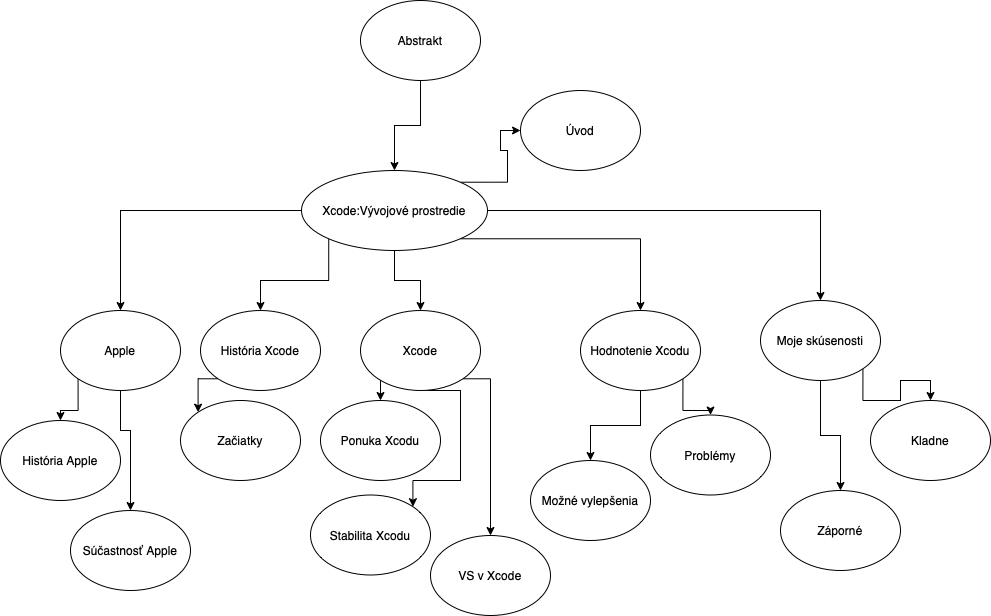
\includegraphics[width=1.1\textwidth]{diagram_kapitol.png}
\end{center}

\newpage
\renewcommand*\contentsname{Obsah}
\tableofcontents

\newpage
\section{Úvod}

\newpage
\section{Apple}
\subsection{História Apple}
Spoločnosť založili dvaja technologickí nadšenci Steve Jobs a Steve Wozniak,  ktorí sa spoznali vo veku 16 a 21 rokov.  K nápadu vytvoriť svoj prvý vlastný počítač prišli tak,  že Jobs za myšlienkou zarobiť si prijal objednávku na 50 počítačov od miestnej počítačovej predajne.  Po dlhom presviedčaní svojho kamaráta Wozniaka spolu s niekoľkými nadšencami tak vytvorili svoj prvý počítač Apple 1.  Počítače pre objednávku vytvorili na čas,  spolu bolo vyrobených až 200ks Apple 1.  \par
Myšlienka výroby osobných počítačov sa dvom nadšencom zapáčila natoľko,  že si chceli založiť firmu.  Jediný problém boli však peniaze,  ktorých zháňanie mal na starosti Steve Jobs.  Banky im požičať nechceli,  sami tak veľký kapitál nemohli pokryť.  Steve hľadal až stretol Mika Markkulu,  ktorý s nimi podpísal bankovú pôžičku na 250 000 dolárov a spolu tak založili v roku 1976 spoločnosť Apple Computer, Inc.

\subsection{Súčastnosť Apple}
Apple je v súčasnosti americký technologický gigant sídliaci v Silicon Valley v kalifornskom meste Cupertino,  USA.  Podľa portálu Forbes sa jedná o spoločnosť s najväčšou trhovou hodnotou na svete (2021).  Spoločnosť sa zameriava hlavne na výrobu počítačov Mac,  smartfónov,  tabletov a podobných smart zariadení ale aj na výrobu operačných systémov ako macOS,  iOS,  programov ale aj vývojových prostredí Xcode.

\newpage
\section{História Xcode}
\subsection{Začiatky}
Prvá verzia Xcode bola publikovaná na jeseň 2003 ako Xcode 1.0,  podľa developer.apple.com bola založená na nástroji Project Builder ale narozdiel od neho mala aktualizované používateľské rozhranie,  distribuovanú podporu zostavy a indexovanie kódu.  Ďalšie vydanie,  verzia 1.5 malo vylepšené dokončovanie kódu a ladenie.  \par
Druhá verzia bola predstavená v roku 2005 spolu s macOS X v10.4,  ponúkala vylepšené indexovanie kódu pre programovací jazyk Java a zároveň ponúkala podporu pre jazyk Ant.  S druhou verziou prišiel aj nástroj na čítanie oficiálnej dokumentácie firmy Apple.

\newpage
\section{Xcode}
\subsection{Ponuka Xcodu}
Vývojom prostredia Xcode prichádzali nové programovacie jazyky,  ktoré toto prostredie podporovalo.  Vsúčasnosti Xcode ponúka podporu pre programovacie jazyky ako C,  C++,  Objective-C,  Objective-C++,  Java,  AppleScript,  Python,  Ruby alebo Swift.  Vďaka podpore od tretích strán ale aj jazyky ako GNU Pascal alebo C\#.  Xcode tiež ako jediné IDE vie skompilovať a nainštalovať aplikáciu vo vývoji určenú pre operačné systémy od spoločnosti Apple použitím iOS SDK,  tvOS SDK,  watchOS SDK alebo macOS SDK.

\subsection{Stabilita Xcodu}
Xcode je na rozdiel od iných vývojových prostredí náročný na výpočtový výkon a úložisko.  Tento problém sa preukazuje hlavne pri vývoji náročnejších a komplexných projektov.  \par
Pri vývoji aplikácii v Xcode je podľa testovania github používateľa ashfurrow dôležitejší výpočtový výkon procesora ako kapacita RAM.  V jeho rebríčku môžeme vidieť, že ani pomerne veľká kapacita operačnej pamäte (32GB) neurýchlila čerstvú kompiláciu aplikácie tak,  ako ju urýchlil vyšší výpočtový výkon procesora (Apple M1).  \par
Rovnako tak je Xcode náročný aj na úložný priestor.  Inštalačný súbor vývojového prostredia Xcode má sám o sebe približne 10GB,  no po nainštalovaní viacerých súčastí sa táto hodnota môže zväčšiť až na 50GB.

\subsection{VS v Xcode}

\newpage
\section{Hodnotenie Xcode}
Podľa viacerých recenzií na stránke g2.com je Xcode „veľmi dobré IDE s veľa chybami“.  Xcode je veľmi jednoduchý na používanie pre začiatočníkov a je ľahké naučiť sa ho používať za pár dní.

\subsection{Problémy}
Viacerým užívateľom vadí,  že Xcode je jediné užívateľské prostredie,  ktoré dokáže kompilovať aplikácie pre iOS,  vývojár si teda nevie vybrať iné IDE,  kde by testoval aplikácie pre iOS.  Tento problém pramení skôr z politiky spoločnosti Apple ako zo samotného vývojového prostredia.  \par
Používateľom tiež vadí debugger a slabý popis problémov v logovacích súboroch v porovnaní s Android Studiom (AS).  Debugovanie cez bezdrôtovú sieť je v porovnaní s AS veľmi pomalé.  \par
Problémom sú aj vysoké nároky na ukladací priestor.  Xcode potrebuje minimálne 10GB úložného priestoru,  čo je pre niektoré zariadenia veľmi veľké.
Aj napriek týmto problémom je Xcode niečo,  čo vývojári potrebujú ak chcú programovať aplikácie pre Apple zariadenia,  ktoré majú v súčasnosti pomerne veľké zastúpenie na trhu.

\subsection{Možné vylepšenia}

\newpage
\section{Moje skúsenosti}
\subsection{Kladné}
\subsection{Záporné}

\newpage
\renewcommand\refname{Referencie}
\bibliography{refs}{}
\bibliographystyle{plain}
\nocite{*}

\end{document}